\chapter{Corriente alterna trifásica}

\section{Enunciado}

\begin{minipage}{0.6\textwidth}
  En el sistema de la figura de secuencia de fases directa y frecuencia
  $f=\qty{60}{\hertz}$, se dispone de un receptor equilibrado con una
  potencia total $P_T=\qty{51984}{\watt}$ factor de potencia de $0.6$ en
  retraso. Sabiendo que el amperímetro marca
  $\qty[parse-numbers=false]{76\sqrt{3}}{\ampere}$, determinar:
  \begin{enumerate}
  \item Medida delos vatímetros 1 y 2.
  \item Valor de la impedancia $\overline{Z}$ en forma módulo-argumento.
  \item Valor de la capacidad mínima para mejorar el factor de potencia
    a $0.95$ en retraso.
  \item Valor de la impedancia equivalente en estrella.
  \end{enumerate}
\end{minipage}
\begin{minipage}{0.4\textwidth}
  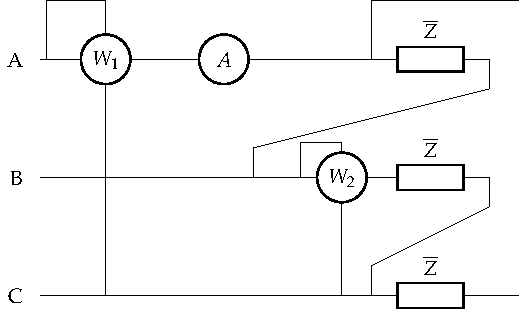
\includegraphics[width=0.9\textwidth]{figuras/ej1_CAtrif.pdf}
\end{minipage}

\subsection{Solución}

Para solucionar las preguntas en este problema, antes de calcular
nada, podemos extraer la siguiente información del enunciado:
\begin{itemize} % para incluir viñetas
\item Se tiene una sola carga trifásica equilibrada de valor $Z$ y con
  $\cos{\phi}=0,6\rightarrow \qty{53.13}{\degree}$ en retraso. Esto
  significa que la impedancia $\overline{Z}$ es de carácter inductivo
  y su potencia reactiva será positiva.
\item Se tiene una secuencia de fases directa ABC. Esto significa que
  el sistema de alimentación tiene las siguientes tensiones de línea:
  $\overline{U}_{AB}=\qty[parse-numbers=false]{U_{AB}\phase{\ang{120}}}{\volt}$,
  $\overline{U}_{BC}=\qty[parse-numbers=false]{U_{BC}\phase{\ang{0}}}{\volt}$
  y
  $\overline{U}_{CA}=\qty[parse-numbers=false]{U_{CA}\phase{\ang{-120}}}{\volt}$. Así
  pues, las tensiones de fase son:
  $\overline{U}_{A}=\qty[parse-numbers=false]{U_{A}\phase{\ang{90}}}{\volt}$,
  $\overline{U}_{B}=\qty[parse-numbers=false]{U_{B}\phase{\ang{-30}}}{\volt}$
  y
  $\overline{U}_{C}=\qty[parse-numbers=false]{U_{C}\phase{\ang{-150}}}{\volt}$.
\item Anotamos la frecuencia de red de valor $\qty{60}{\hertz}$ por si
  hemos de calcular alguna reactancia inductiva y/o capacitiva.
\item La potencia activa total que demanda el triángulo de impedancia
  $\overline{Z}$ es de valor $P_T=\qty{51984}{\watt}$. De este valor,
  sacamos como conclusión que cada impedancia $\overline{Z}$ del
  triángulo consume un tercio de dicha potencia activa al ser un
  receptor equilibrado.
\item El vatímetro $W_2$ está conectado midiendo la intensidad
  $\overline{I}_{BC}$ y la tensión $\overline{U}_{BC}$, es decir, nos
  da el valor de la potencia activa que disipa la fase BC del
  triángulo, cuyo valor ya sabemos que es:
  \[
    W_2=\dfrac{P_T}{3}=\dfrac{51984}{3}=\qty{17328}{\watt}
  \]
\item El amperímetro dispuesto en la línea A mide el valor eficaz de
  $\qty[parse-numbers=false]{76\sqrt{3}}{\ampere}$. Esto significa que,
  al tener un receptor equilibrado conectado en triángulo, las
  intensidades por las otras dos líneas B y C tienen el mismo valor de
  intensidad de valor eficaz de
  $\qty[parse-numbers=false]{76\sqrt{3}}{\ampere}$.
\item También, al ser un receptor equilibrado conectado en triángulo,
  las intensidades $\overline{I}_{AB}$, $\overline{I}_{BC}$ e
  $\overline{I}_{CA}$ que circulan dentro del triángulo, toman por
  valor eficaz:
  \[
    \dfrac{76\sqrt{3}}{\sqrt{3}}=\qty{76}{\ampere}
  \]
\item Los argumentos de las intensidades dentro de triángulo se pueden
  obtener del propio enunciado. Cada intensidad $\overline{I}_{AB}$,
  $\overline{I}_{BC}$ e $\overline{I}_{CA}$ retrasa
  $\ang{53,13}$ a las tensiones $\overline{U}_{AB}$,
  $\overline{U}_{BC}$ y $\overline{U}_{CA}$ correspondientes, es
  decir, la intensidad $\overline{I}_{AB}$ tiene un argumento de valor
  $120-53,13=\ang{66,87}$, la intensidad $\overline{I}_{BC}$
  tiene un argumento de valor $0-53,13=\ang{-53,13}$ y la
  intensidad $\overline{I}_{CA}$ tiene un argumento de valor
  $-120-53,13=\ang{-153,13}$.
\item Los argumentos de las intensidades de línea también se pueden
  obtener del propio enunciado. Cada intensidad $\overline{I}_A$,
  $\overline{I}_B$ e $\overline{I}_C$ retrasa $\ang{53,13}$ a
  las tensiones del sistema de alimentación $\overline{U}_A$,
  $\overline{U}_B$ y $\overline{U}_C$ correspondientes, es decir, la
  intensidad $\overline{I}_A$ tiene un argumento de valor
  $90-53,13=\ang{36,87}$, la intensidad $\overline{I}_B$ tiene
  un argumento de valor $-30-53,13=\ang{-83,13}$ y la
  intensidad $\overline{I}_C$ tiene un argumento de valor
  $-150-53,13=\ang{-203,13}$.
\end{itemize}

Tras estas consideraciones, se pueden iniciar los cálculos necesarios
para responder a las preguntas del problema:
\begin{enumerate}
\item Medida de los vatímetros 1 y 2.
    
  La lectura del vatímetro 1, según está conectado, es la siguiente:
  \[ [W_1]=\Re(\overline{U}_{AC}\cdot \overline{I} _A)=U_{AC}\cdot I_A\cdot
    \cos(\langle \overline{U}_{AC}, \overline{I}_A \rangle)
  \]

  Se desconoce el módulo de la tensión $\overline{U}_{AC}$. Se calcula
  a partir del vatímetro 2 cuya lectura es de
  $[W_2]=\qty{17328}{\watt}$:
  \begin{align*}
 [W_2] &=\Re(\overline{U}_{BC} \cdot \overline{I}_{BC})=U_{BC}\cdot
    I_{BC}\cdot \cos(\langle \overline{U_{BC}},
         \overline{I_{BC}}\rangle)\\
    17328&=U_{BC}\cdot 76\cdot
    0.6\Rightarrow U_{BC}=\qty{380}{\volt}
  \end{align*}
  Por tanto, al ser un sistema equilibrado ($U_{AB}=U_{BC}=U_{CA}$), y
  sabiendo que
  $\overline{U}_{AC}=-\overline{U}_{CA}=U_{CA}\phase{-120+180}=\qty[parse-numbers=false]{380\phase{\ang{60}}}{\volt}$,
  la lectura del vatímetro 1:
  \[ [W_1]=\Re(\overline{U}_{AC}\cdot \overline{I}_A)=U_{AC}\cdot I_A\cdot
    \cos(\langle \overline{U}_{AC}, \overline{I}_A \rangle)=380\cdot
    76\sqrt{3}\cdot \cos(\langle60;36.87\rangle)=\qty{46001}{\watt}
  \]

\item Valor de la impedancia $\overline{Z}$ en forma módulo-argumento.

  Al conocer ya el valor de la tensión a la que está alimentada y la
  intensidad que circula por ella, se obtiene su valor fácilmente a
  partir de la ley de Ohm:
  \[
    \overline{Z}=\dfrac{\overline{U}_{AB}}{\overline{I}_{AB}}=\dfrac{380\phase{120}}{76\phase{66.87}}=\qty[parse-numbers=false]{5\phase{\ang{53.13}}}{\ohm}
  \]

\item Valor de la capacidad mínima para mejorar el factor de potencia
  a $0.95$ en retraso.




\item Valor de la impedancia equivalente en estrella.


\end{enumerate}

\section{}
% poner aqui el ENUNCIADO DEL PROBLEMA

\subsection{}

% poner aqui la SOLUCION DEL PROBLEMA

%%% Local Variables:
%%% mode: latex
%%% TeX-master: "Problemas_TC"
%%% ispell-local-dictionary: "castellano"
%%% End:
